\documentclass[svgnames]{article}
\usepackage{tikz}  					% use "amsart" instead of "article" for AMSLaTeX format
\usepackage{geometry}                		% See geometry.pdf to learn the layout options. There are lots.
\geometry{letterpaper} 
                  						% ... or a4paper or a5paper or ... 
%\geometry{landscape}                		% Activate for rotated page geometry
%\usepackage[parfill]{parskip}    		% Activate to begin paragraphs with an empty line rather than an indent
\usepackage{graphicx}	
\newtheorem{theorem}{Theorem}		% Use pdf, png, jpg, or eps§ with pdflatex; use eps in DVI mode
	
%images

\graphicspath{{img/}}	
	
	
%math							% TeX will automatically convert eps --> pdf in pdflatex		
\usepackage{amssymb}
\usepackage{amsmath}
\usepackage{esint}

%pgfplots & tikz
\usepackage{pgfplots}
\usepackage{comment}

%Figures
\usepackage{float}
\usepackage{caption}
\usepackage{lipsum}





\title{Physics 5B}
\author{deval deliwala}
%\date{}					% Activate to display a given date or no date


\begin{document}
\maketitle
\begin{center}
Adapted from Electricity + Magnetism, 2nd Edition by Purcell 
\end{center}
%\section{}
%\subsection{}

\vspace{60px}

% Electromagnetic wave - black
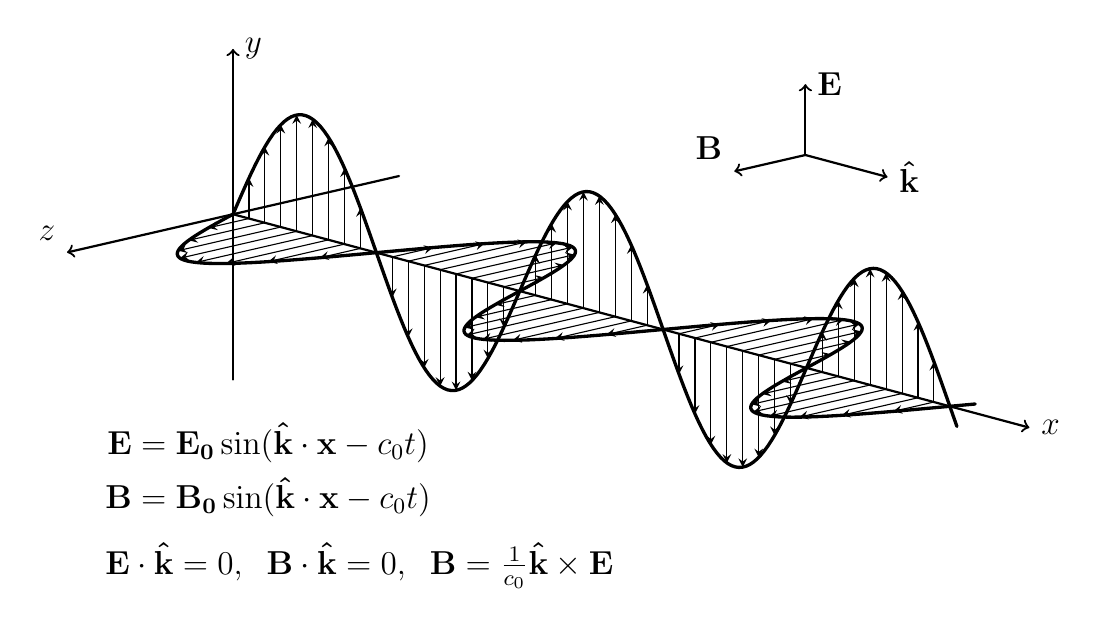
\begin{tikzpicture}[x=(-15:1.2), y=(90:1.0), z=(-150:1.0),
                    line cap=round, line join=round,
                    axis/.style={black, thick,->},
                    vector/.style={>=stealth,->}]
  \large
  \def\A{1.5}
  \def\nNodes{5} % use even number
  \def\nVectorsPerNode{8}
  \def\N{\nNodes*40}
  \def\xmax{\nNodes*pi/2*1.01}
  \pgfmathsetmacro\nVectors{(\nVectorsPerNode+1)*\nNodes}
  
  \def\vE{\mathbf{E}}
  \def\vB{\mathbf{B}}
  \def\vk{\mathbf{\hat{k}}}
  
  % MAIN AXES
  \draw[axis] (0,0,0) -- ++(\xmax*1.1,0,0) node[right] {$x$};
  \draw[axis] (0,-\A*1.4,0) -- (0,\A*1.4,0) node[right] {$y$};
  \draw[axis] (0,0,-\A*1.4) -- (0,0,\A*1.4) node[above left] {$z$};
  
  % SMALL AXES
  \def\xOffset{{(\nNodes-2)*pi/2}}
  \def\yOffset{\A*1.2}
  \def\zOffset{\A*1.2}
  \draw[axis] (\xOffset,\yOffset,-\zOffset) -- ++(\A*0.6,0,0) node[right] {$\vk$};
  \draw[axis] (\xOffset,\yOffset,-\zOffset) -- ++(0,\A*0.6,0) node[right] {$\vE$};
  \draw[axis] (\xOffset,\yOffset,-\zOffset) -- ++(0,0,\A*0.6) node[above left] {$\vB$};
  
  % equation
  \node[above right] at (\xOffset,-0.5*\yOffset,4*\zOffset)
    {$\begin{aligned}
      \vE &= \mathbf{E_0}\sin(\vk\cdot\mathbf{x}-c_0t)\\
      \vB &= \mathbf{B_0}\sin(\vk\cdot\mathbf{x}-c_0t)\\
      \end{aligned}$};
  \node[below right] at (\xOffset,-0.5*\yOffset,4*\zOffset)
    {$\vE\cdot\vk = 0,\;\; \vB\cdot\vk = 0,\;\; \vB = \frac{1}{c_0}\vk\times\vE$};
  
  % waves
  \draw[very thick,variable=\t,domain=0:\nNodes*pi/2*1.01,samples=\N]
    plot (\t,{\A*sin(\t*360/pi)},0);
  \draw[very thick,variable=\t,domain=0:\nNodes*pi/2*1.01,samples=\N]
    plot (\t,0,{\A*sin(\t*360/pi)});
  
  % draw vectors
  \foreach \k [evaluate={\t=\k*pi/2/(\nVectorsPerNode+1);
                         \angle=\k*90/(\nVectorsPerNode+1);
                         \c=(mod(\angle,90)!=0);}]
              in {1,...,\nVectors}{
    \if\c1
      \draw[vector] (\t,0,0) -- ++(0,{\A*sin(2*\angle)},0);
      \draw[vector] (\t,0,0) -- ++(0,0,{\A*sin(2*\angle)});
    \fi
  }
  
\end{tikzpicture}

\newpage
\tableofcontents

\newpage



\section{Electrostatics: Charges and Fields}
\begin{theorem} 
The total charge in an isolated system never changes
\end{theorem}
\begin{theorem}
The electric charges we find in nature come in units of one magnitude only - e, and each particle and antiparticle possess an exact equality of opposite charges. The magnitude of e is 4.8023e-10 esu
\end{theorem}

\subsection{Coulomb's Law} 
\[ \vec{F} = k\frac{q_1q_2}{r^2}\hat{r} \] \\

\begin{center}
\begin{tikzpicture} 
\fill[black] (2,1) circle[radius = 0.1];
\fill[black] (5,4) circle[radius = 0.1];
\draw[-stealth] (2,1) --  (3,2) node[midway, above left] {$\mathbf{+}$};
\draw[-stealth] (5,4) -- (4,3) node[midway, below right]{$\mathbf{-}$}; 


\end{tikzpicture}
\end{center} 

\vspace{20px}

Two stationary electric charges repel or attract each other with a force proportional to the product of the magnitude of the charges and inversely proportional to the square of the distance between them

\[ k = 8.988 \times 10^9 \] 
 
It is customary to introduce a constant $e_0$ with which the same equation is written \\ 

\[ \vec{F} = \frac{1}{4\pi \epsilon_0}\frac{q_1q_2}{r^2}\hat{r} \] \\

In addition, Coulomb's Law is \textit{additive} in its effect. \\

\[ \vec{F}_1 = \frac{1}{4\pi \epsilon_0}\frac{q_1q_2}{r_{12}^2}\hat{r}_{12} + \frac{1}{4\pi \epsilon_0}\frac{q_1q_3}{r_{13}^2}\hat{r}_{13} \] \\

This phenomenon of having a three-charge system and being able to reduce the interactions of each particle into an interaction between two particles and adding them to produce the force on any one of the particles is known as \textit{Superposition} 

\subsection{Energy of a System Never Changes}

\vspace{20px}

\begin{center}
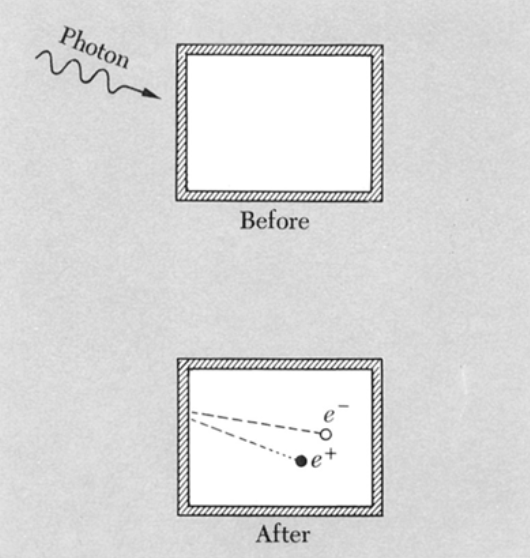
\includegraphics[width = 50mm]{ss3.png}
\end{center} 


\vspace{20px}

Energy is a useful concept in electrostatics because electrical forces are \textit{conservative}, meaning they are path independant and everything is perfectly reversible. \\ 

Consider the work which must be done on a system to bring two charged particles very far apart from one another, to a distance $r_{12}$. \\

\[ W = k \int \text{force} \times \text{distance} = k\int_{r = \infty}^{r_{12}} \frac{q_1q_2}{r^2}\,(-dr) = k\frac{q_1q_2}{r_{12}} \] \\

The reason $dr$ is negative is because the force that has to be applied to move one charge toward the other is equal and \textit{opposite} to the coulumb force. It makes no difference whether we bring $q1$ toward $q_2$ or the other way around. 

Suppose we wish to bring a third charge $q_3$ and move it to a point $P_3$, whose distance from $q_1$ is $r_{31}$ and from $q_2$ is $r_{32}$. The work required is \\

\[ W_3 = - k\int_\infty^{P_3} \vec{F}_3 \cdot \, d\vec{s}  \] \\

Thanks to the additivity of electrical interactions, \\ 
\begin{align*}
-k\int \vec{F}_3 \cdot \, d\vec{s} &= -k\int \vec{F}_{31} + \vec{F}_{32} \cdot d\vec{s} \\
&= -k\int \vec{F}_{31} \cdot d\vec{r} - k\int \vec{F}_{32} \cdot d\vec{r} \\ 
&= k\frac{q_1q_3}{r_{31}} + k\frac{q_2q_3}{r_{32}} 
\end{align*} \\ 

Therefore, the total work done in assembling this arrangement of three charges, $U$ is \\

\[ U = k\frac{q_1q_2}{r_{12}} + k\frac{q_1q_3}{r_{13}} +  k\frac{q_2q_3}{r_{23}} \] \\

This is known as the \textit{electric potential energy} of this particular system. \\

As an example, let us calculate the potential energy of an arrangement of eight negative charges at the corners of a cube, with a positive charge in the center of the cube, with sides length $b$. Suppose each negative charge is an electron (-e) and the central particule carries a charge $2e$. Summing over all pairs, we have \\ 


\begin{center}
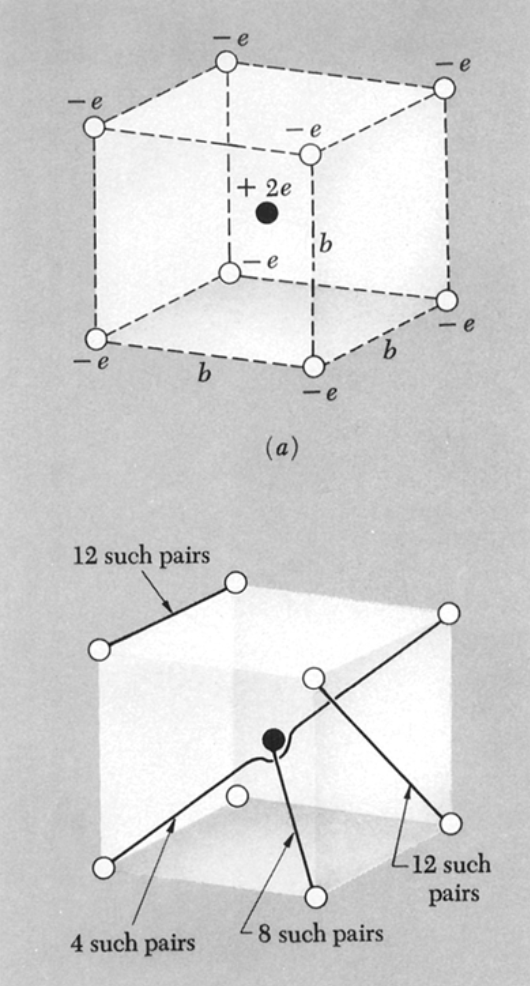
\includegraphics[scale = 0.4]{ss4.png}
\end{center} 


\[ U = \frac{8 (-2e^2)}{\frac{\sqrt{3}}{2}b} + \frac{12e^2}{b} + \frac{12e^2}{\sqrt{2}b} + \frac{4e^2}{\sqrt{3}b} = \frac{4.32e^2}{b} \] \\

A simpler way of calculating potential energy is \\

\[ U = \frac{1}{2}\sum_{j=1}^N \sum_{k\neq j}^N \frac{q_jq_k}{r_{jk}} \]

\subsection{The Electric Field} 

\vspace{20px}

\begin{center}
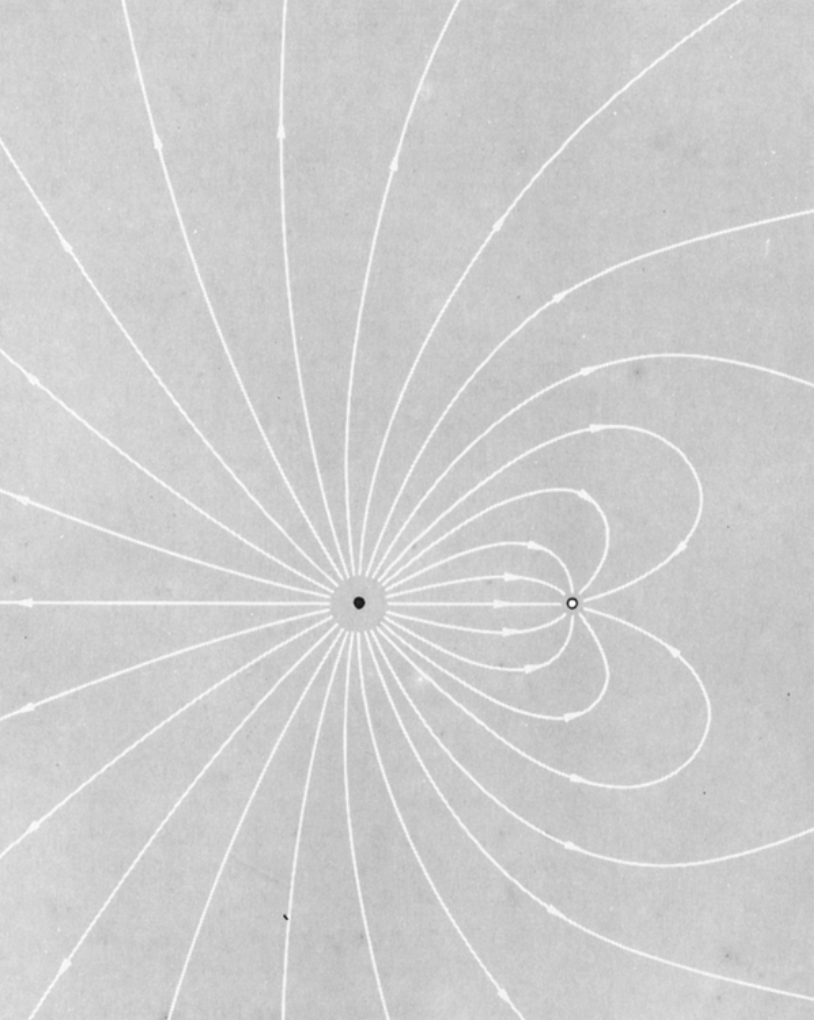
\includegraphics[width = 50mm]{ss7.png}
\end{center} 


\vspace{20px}

The force on a charge in the vicinity of $N$ other charges is given by \\ 

\[ \vec{F}_0 = \frac{1}{4\pi\epsilon_0} \ \sum_{j=1}^N \frac{q_0q_j}{r_{0j}^2}\hat{r}_{0j} \]

If we divide out $q_0$ we obtain a vector function dependent on the structure of the original system of charges. We call this function the \textit{electric field} \\ 

\[ \vec{E}(x,y,z) = \frac{1}{4\pi\epsilon_0}\sum_{j=1}^N \frac{q_j}{r_{0j}^2}\hat{r}_{0j} \] \\


\subsection{Charge Distributions} 

A volume distribution of charge is described by a scalar charge-density function $\rho$. If the source of an electric field is to be a continuous charge distribution rather than point charges, \\

\[ \vec{E}(x,y,z) = \frac{1}{4\pi\epsilon_0} \iiint \frac{\rho(x',y',z')}{r^2} \hat{r} \, dx'dy'dz' \] \\

This integral gives the electric field at $(x,y,z)$ produced by charges at other points $(x',y',z')$

\subsection{Flux}
  

\textit{Flux} describes the relation between the electric field and its sources. It describes the ``rate of flow'' of a vector field through an area. For an electric field, \\

\[ \Phi = \sum_{\text{All j}} \vec{E}_j \cdot \vec{a}_j \] \\

which ultimately becomes \\ 

\[ \oiint_\text{entire surface} \vec{E} \cdot d\vec{a} \] \\ 

As an example, the flux of a point charge $q$ through a sphere of a radius $r$ centered on the poitn charge is given by

\[ \Phi = E \times \text{total area} = \frac{q}{r^2} \times 4\pi r^2 = 4\pi q \] 

\subsection{Gauss's Law} 

\begin{theorem}
The total flux through a closed surface is 0, and the flux of an electric field through \textit{any} closed surface enclosing a point charge $q$ is $4\pi q$ 
\end{theorem} 

The situation is now ripe for superposition. Flux is an additive quantity is away. If we have a number of sources $q_1,q_2,...,q_N$, the fields of which would be $E_1,E_2,...,E_N$, the flux $\Phi$ through some surface $S$ in the actual field can be written as \\

\[ \Phi = \int_S \vec{E} \cdot d\vec{a} = \int_S (E_1 + E_2 + ... + E_N) \cdot d\vec{a} \] \\

Therefore, every charge $q$ inside the surface contributes exactly $4\pi q$ to the surface integral and all charges outside contribute nothing. We have arrived at Gauss's Law \\ 

\[ \textbf{Gauss's Law} \rightarrow  \oiint \vec{E} \cdot d\vec{a} = 4\pi \sum_i q_i = 4\pi \iiint \rho \, dv =  \frac{Q}{\epsilon_0} \] \\ 


\textbf{Note*} \\

Coulombs Law tells us how to derive the electric field if the charges are given; with Gauss's Law we can determine how much charge is in any region if the field is known. 

\subsection{Field of a Spherical Charge Distribution} 

\vspace{20px}

\begin{center}
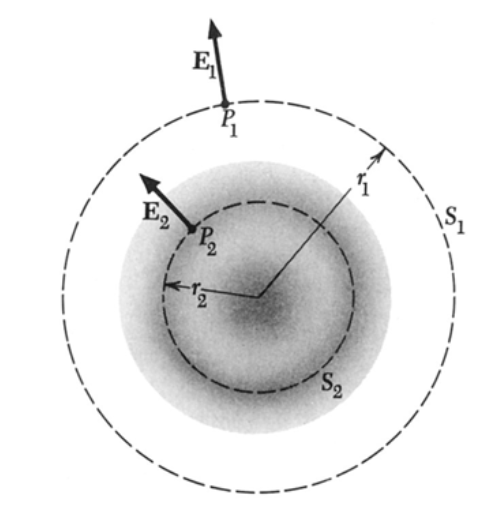
\includegraphics[width=50mm]{ss6.png}
\end{center}


\vspace{20px}

We can use Gauss's Law to find the electric field of a spherically symmetrical distribution of charge, where $\rho$ depends only on the radius from a central point \\


\begin{align*}
\oiint \vec{E} \cdot d\vec{A} &= \frac{Q}{\epsilon_0} \\
\vec{E} A &= \frac{\rho V}{\epsilon_0} \\ 
\vec{E} &= \frac{\rho V}{4 \pi r^2 \epsilon_0} \\
\vec{E} &= \frac{\rho (\frac{4}{3}\pi R^3)}{4 \pi r^2 \epsilon_0}
\end{align*}\\
\begin{center}


\textbf{for a spherical shell,}
\end{center}

\[ \Phi = \vec{E} \times \text{area} = 4\pi r^2 E \] 

\begin{align*} 
\oiint \vec{E} \cdot d\vec{a} &= \frac{Q}{\epsilon_0} \\
\vec{E}A &= \frac{4\pi r_0^2 \sigma}{\epsilon_0} \\ 
\vec{E} &= \frac{4\pi r_0^2 \sigma}{4\pi r^2 \epsilon_0} \\ 
\vec{E} &= \frac{r_0^2 \sigma}{r^2 \epsilon_0}
\end{align*} \\


Indeed, the Electric Field inside a spherical shell of charge is 0 because the charge enclosed is 0 \\

\subsection{Field of a Line Charge} 

\vspace{20px} 

\begin{center}
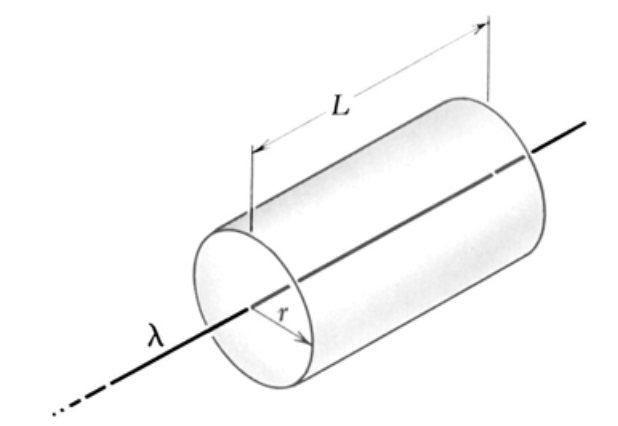
\includegraphics[width = 50mm]{screenshot.png}
\end{center} 


\vspace{10px}


A long, straight, charged wire, if we neglect thickness, can be characterized by $\lambda$, the linear charge density. Using Gauss's Law, surround a segment of the line of charge with a closed circular cylinder of length $L$ and radius $r$, and consider the flux through this surface. \\

The symmetry guarantees that the field is radial, so the flux through the ends of the cylinder are zero. The flux through the cylindrical surface is simply the area, $2\pi rL$, times $E_r$, the field at the surface. Since the charge enclosed by the surface is just $\lambda L$, Gauss's Law gives us \\

\[ \Phi = \frac{\lambda L}{\epsilon_0} = 2\pi r L E_r = 4 \pi \lambda L  \]  

Therefore, \\

\[ E_r = \frac{2 \lambda}{r} \] 

\subsection{Field of an Infinite Flat Sheet of Charge}

\vspace{20px} 

\begin{center}
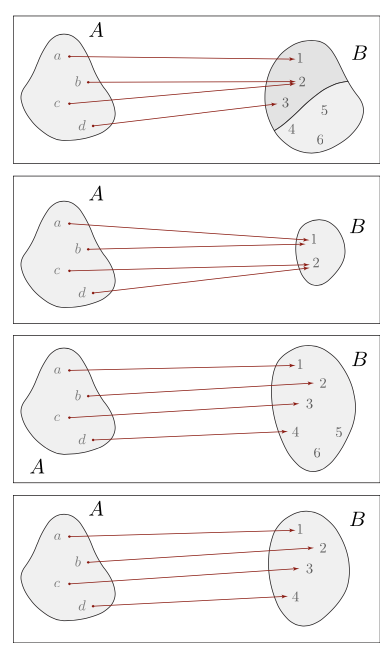
\includegraphics[width = 50mm]{ss.png}
\end{center} 


\vspace{20px}

Let the surface charge density be denoted by $\sigma$, and let there exist a cylinder, perpendicular through the infinite sheet, with sides $P'$ and $P$ on either side. The outward flux is found only one the ends. Therefore

\[ AE_P + AE_{P'} = 2AE_P \] 

The charge enclosed is $A\sigma$ Hence, 

\begin{align*}
&\oiint \vec{E} \cdot dA = \frac{q_{enc}}{\epsilon_0} \\ 
&\vec{E} A = \frac{\sigma A}{\epsilon_0} \\
&\vec{E} = \frac{\sigma A}{\epsilon_0} 
\end{align*} \\

We see that the field strength is independent of $r$, thus if one were to build an infinite flat sheet of charge, the electric field would permeate throughout the universe at the exact same strength. 

\subsection{The Force on a Layer of Charge}

\vspace{20px}

To calculate the electric force experienced by the charges that make up the spherical distribution, we must think about the force on a small element of charge $dq$, such as a small patch of area $dA$ with charge $dq = \sigma dA$. 

\[ d\vec{F} = \vec{E} dq = \vec{E} \sigma dA \]

The electric field we use, which will not be justified (it's in the textbook) is the average of the electric field on the sphere and outside the sphere. \\ 
\begin{align*} 
 dF &= \frac{1}{2} (4\pi \sigma + 0)\sigma dA = 2\pi \sigma^2 dA\\
 dF &=  E \rho dx \\
 F &= \int_0^{x_0} E\rho \, dx \\
 F &= \frac{1}{4\pi} \int_{E_1}^{E_2} E \, dE = \frac{1}{8\pi} (E_2^2 - E_1^2)
 \end{align*} \\
 
 Since $E_2 - E_1 = 4\pi \sigma$, 
 
 \[ F = \frac{1}{2}(E_1 + E_2)\sigma \] 
 
 \subsection{Energy associated with the electric field} 
 
 The derivation for the potential energy $U$ is in the textbook, but basically since $F = \frac{dU}{dt}$
 
 \[ F = \frac{E^2}{8\pi} \rightarrow U = \frac{1}{8\pi} \int_\text{entire field} E^2 \, dv \] \\
 
 $E^2$ is a scalar quantity, $E^2 = \vec{E} \cdot \vec{E}$ \\
 
 Consider two charged particles, a proton and a negative \textit{pion}. Let $E_p$ be the electric field of the proton and $E_\pi$ that of the pion. The total electric field is thus, $\vec{E} = \vec{E}_p + \vec{E}_\pi$ and $\vec{E} \cdot \vec{E} = E_p^2 + E_\pi^2 + 2\vec{E}_p \cdot \vec{E}_\pi$. Therefore, the energy in the electric field of this two-particle system is 
 
 \begin{align*} 
 U &= \frac{1}{8\pi} \int E^2 dv \\
 &= \frac{1}{8\pi} \int E_p^2 \, dv + \frac{1}{8\pi} \int E_\pi^2 \, dv + \frac{1}{4\pi} \int \vec{E}_p \cdot \vec{E}_\pi \, dv
 \end{align*}
 
 \vspace{20px}
 \subsection{Chapter One Problems} 
 
 \subsubsection{1.1} 
 
 Compare the electrostatic repulsion force in 2 \textit{nucleons} to gravity. Let the nucleon mass be $1.6 \times 10^{-24}$ gm, and the gravitational constant $G$ be $ 6.7 \times 10^{-8} \frac{\text{cm}^3}{\text{gm sec}^2}$. Let the distance be $10^{-13} cm$. 
 
 \vspace{20px} 
 
 \textbf{Gravitational Attraction} 
 
 \begin{align*} 
 \vec{F} &= \frac{Gm_1m_2}{r^2} \\
 \vec{F} &= \frac{(6.7 \times 10^{-8}) (1.6 \times 10^{-24})^2}{(10^{-13})^2} \\
 & = 1.7152 \times 10^{-29} N 
 \end{align*}
 
 \vspace{10px} 
 
 \textbf{Electrostatic Attraction} 
 \begin{align*} 
 \vec{F} &= \frac{kq_1q_2}{r^2} \\
 \vec{F} &= \frac{(8.988 \times 10^{9})1^2}{(10^{-13})^2} \\
 & = 8.988 \times 10^{35} N
 \end{align*}
 
\vspace{10px} 

\[ 10^{35} >> 10^{-29} \]

\newpage

\section{The Electric Potential} 

\subsection{Line Integrals of the Electric Field} \mbox{} \\

Suppose that $\vec{E}$ is the field of some stationary distribution of electric charges. Let $P_1$ and $P_2$ denote two points anywhere in the field. The line integral of $E$ between the two points is 
\[ \int_{P_1}^{P_2} \vec{E} \cdot d\vec{s} \] \\

A line integral is essentially just summing up an infinite number of small vectors tangent to the line from $P_1$ to $P_2$ \\ 

\begin{center}
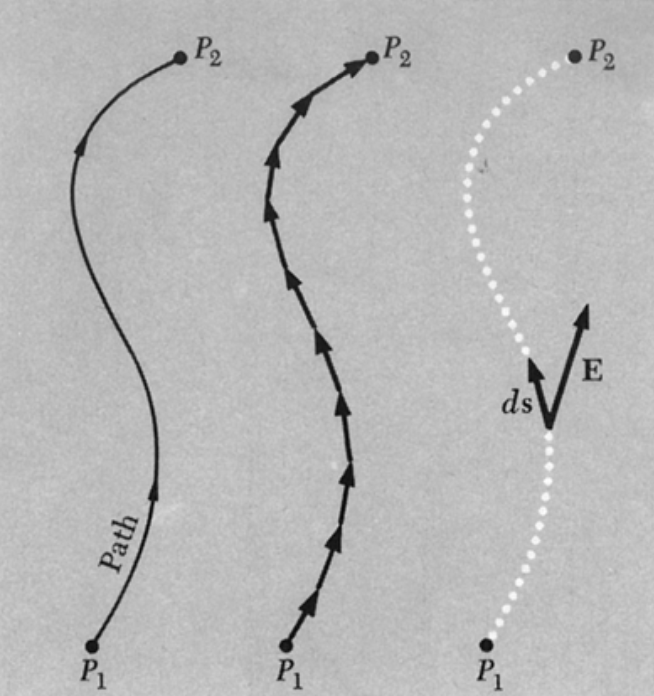
\includegraphics[width = 50mm]{ss8.png}
\end{center} 

Let us consider the field of a point charge $q$ and some paths running from a point $P_1$ to $P_2$ in that field. Let $r_1$ be the radius from $q$ to $P_1$ and $r_2$ the radius from $q$ to $P_2$ \\ 

\[ \int_C \vec{E} \cdot d\vec{s} = \int_{r_1}^{r_2} \frac{q}{r^2} \, dr = q\left(\frac{1}{r_1} - \frac{1}{r_2} \right) \] \\

This equation holds for all paths between $P_1$ and $P_2$, the vector field $\vec{E}$ is \textit{path indepenent}. In the case that paths are all closed curves, \\


\[ \int_C \vec{E} \cdot d\vec{s} = \vec{0} \] \\

\subsection{Potential Difference and the Potential Function} \mbox{} \\

Because the line integral of an electrostatic field is path independent, we can use it to define a scalar quantity, $\phi_{21}$, without specifying any particular path: 

\[ \phi_{21} = -\int_{P_1}^{P^2} \vec{E} \cdot d\vec{s} \] \\

$\phi_{21}$ is the work per unit charge done in moving a positive charge from $P_1$ to $P_2$ in the electric field $\vec{E}$. We call it the electric potential difference between the two points. \\ 
Potential Difference is measured in \textbf{volts}, where one joule of work is required to move a charge of one coulomb through a potential difference of one volt. \\
If $P_1$ is fixed at some reference position, then $\phi_{21}$ becomes a function of $P_2$, that is, a function of coordinates $x, y, z$. We can write it as $\phi(x, y, z)$. Once the vector field $\vec{E}$ is given, the potential function $\phi$ is determined, except for a certain constant from the choice of $P_1$. \\ \\

\textbf{Example} \\
Find the potential associated with the electric field $\langle Ky, Kx, 0 \rangle$ with $K$ a constant. Since $E_z = 0$, the potential is only determined by the $xy$ plane. Let $x_1, y_1$ be the coordinates of $P_1$ and $x_2, y_2$ the coordinates of $P_2$. It is convenient to make $P_1$ the origin. 

\begin{align*} 
\phi(x_2, y_2) = -\int_{(0,0)}^{(x_2,y_2)} \vec{E} &\cdot d\vec{s} \\ 
& = - \int_{(0,0)}^{(x_2, 0)} E_x \, dx - \int_{(x_2, 0)}^{(x_2, y_2)} E_y \, dy 
\end{align*} \\

The first of the two integrals on the right is 0, since $E_x$ is zero along the x axis. 

\[ -\int_{(x_2, 0)}^{(x_2, y_2)} E_y \, dy = -\int_0^{y_2} Kx_2\,dy = -Kx_2y_2 \] \\

Therefore, 

\[ \phi = -Kxy \] \\

for the potential at any point $(x,y)$ in this field, with 0 potential at the origin. Any constant could be added to this. \\ \\ 

We must be careful not to confuse the potential $\phi$ associated with a given field $\vec{E}$ with the potential \textbf{energy} of a system of charges. The potential energy, $U$ of a system of charges is the total work required to assemble it, starting with all the charges an infinite distance apart. The electric potential $\phi(x, y, z)$ associated with the field is the work per unit charge required to move a unit positive test charge from some chosen reference point to the point $(x, y, z)$ in the field of that structure of charges. \\

\subsection{Derivation of the Field from the Potential}  \mbox{} \\ 

Given the electric field, we can find the electric potential function. But we can also derive the electric field from the potential function. \\

\[d\vec{\varphi} = \frac{\partial \varphi}{\partial x} \, \hat{i} + \frac{\partial \varphi}{\partial \varphi}{\partial y} \, \hat{j} + \frac{\partial \varphi}{\partial x} \, \hat{k} \] \\

In addition, from the definition of $\varphi$, the change can also be represented as \\

\[ d\varphi = - \vec{E} \cdot d\vec{s} \] \\

Thus, if we identify $\vec{E} = - \nabla \varphi$, both equations become identical. So the electric field is the negative of the gradient of the potential:\\

 \[ \vec{E} = - \nabla \varphi \] \\
 
 The minus sign came in because the electric field points from a region of positive potential towards a region of negative potential, but the vector $\nabla \varphi$ is defined so that it points in the direction of increasing $\varphi$ from the definition of the gradient. \\
 
 \subsection{Potential of a Charge Distribution}
 
 We already know the potential that goes with a single point charge, because we calculated the work required to bring one charge into the neighborhood of another before. The potential of any point, in the field of an insolated point charge $q$ is just $k\frac{q}{r}$, where $r$ is the distance from the point in question to the source $q$, and where we have assigned 0 potential to be infinitely far away.  \\
 
 Superposition must work for potentials as well. Thus if we have several sources, the potential function is simply the sum of the potential functions that we would have for each of the sources present alone - \textit{providing} we make a consistent assignment of the zero potential in each case. Therefore, 
 
 \[ \varphi(x, y, z) = \iiint_\text{all sources} \frac{\rho (x', y', z')}{r} \, dx'dy'dz' \] \\
 
 where $r$ is the distance from the volume element $dx', dy', dz'$ to the point $(x, y, z)$. That is, 
 
 \[ r = [(x-x')^2 + (y-y')^2 + (z-z')^2 ]^{1/2} \] \\
 
 Notice the difference between this integral and the integral for the electric field of a charge distribution. Here we have $r$ in the denominator, not $r^2$, and the integral is a scalar not a vector. From the scalar potential function we can always find the electric field 
 
 \subsection{Potential of two point charges} 
 
 Consider a very simple example, the potential of two point charges. A positive charge of 12 esu is located 3cm away from a negative charge of -6 esu. The potential at any point in space is the sum of the potentials due to each charge alone. No vector addition is involved here, only the algebraic addition of scalar quantities. 

\begin{center}
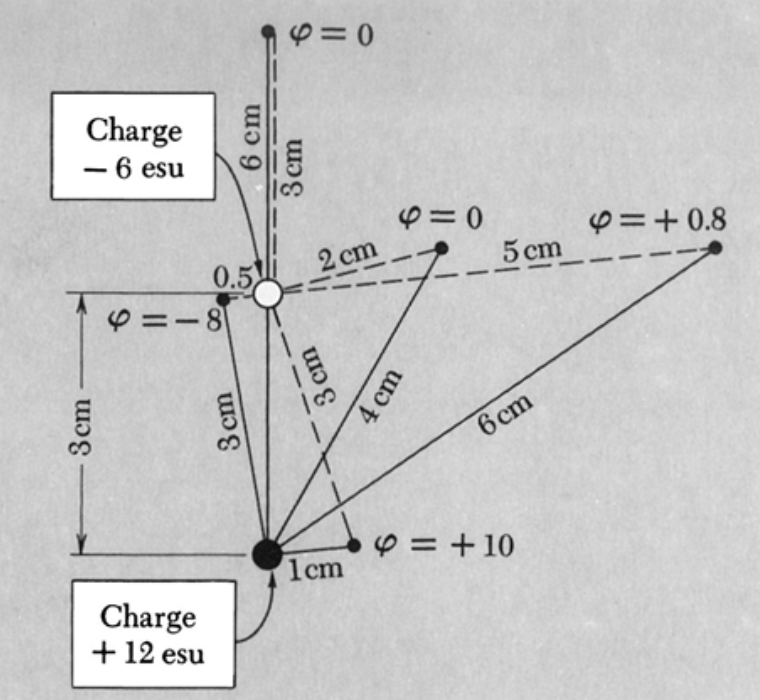
\includegraphics[width = 50mm]{ss9.png}
\end{center} 

\[ \phi = k\sum_{i=1}^N \frac{q_i}{r} \] \\

Therefore the potential at a point 6cm from the positive charge and 5cm from the negative charge is, 

\[
k (\frac{12}{6} - \frac{6}{5}) = 0.8 \times k
\]

\subsection{Potential of a long charged wire} 

To see how to calculate electric potential for an infinitely long charged wire, let us arbitrarily choose a reference point $P_1$ at a distance $r_1$ from the wire. Then to carry a charge from $P_1$ to any other point $P_2$ at a distance $r_2$, requires the work per unit positive charge 

\begin{align*} 
\varphi_{21} &= -\int_{P_1}^{P_2} \vec{E} \cdot d\vec{s} = \int_{r_1}^{r_2} \frac{2\lambda}{r} \, dr \\
&= -2 \lambda \ln r_2 + 2\lambda \ln r_1 
\end{align*} \\

This shows that the electric potential for the charged wire can be taken as 

\[ \varphi = 2\lambda \ln \vec{r} + \text{const.} \] \\

The constant, $2\lambda \ln r_1$ in this case, has no effect when we take $-\nabla \varphi$ to get back to the electric field $\vec{E}$. In this case, 

\[ -\nabla \varphi = -\hat{r} \frac{d \varphi}{dr} = \frac{2\lambda}{r} \hat{r} \] \\

\subsection{Potential of a Uniformly Charged Disk} 

As a start, let us find the potential at some point $P_1$ on the axis of symmetry. 

\begin{center}
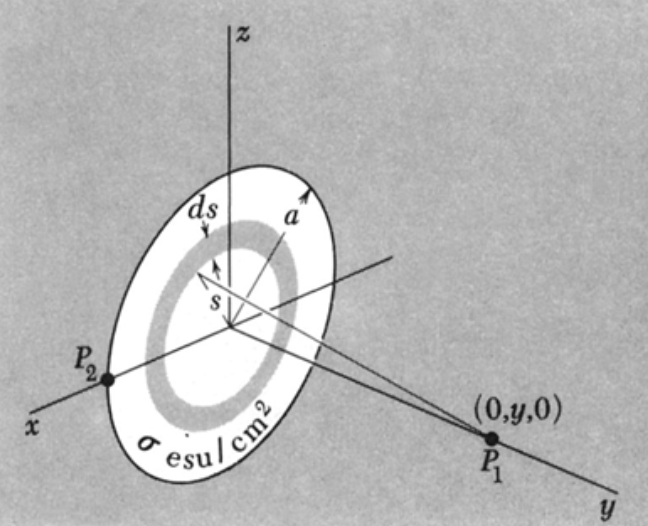
\includegraphics[width = 50mm]{ss10.png}
\end{center} 

All charge elements in a thin, ring-shaped segment of the disk lie at the same distance from $P_1$. If $s$ denotes the radius of such an annular segment and $d\vec{s}$ its width, its area is $2\pi s ds$. The amount of charge it contains is $dq$, which is therefore $\sigma 2\pi s ds$. All parts of this ring are the same distance away from $P_1$, namely $r = \sqrt{y^2 + s^2}$, where the y-axis is the axis of symmetry, so the contribution of the ring to the potential at $P_1$, is $dq / r$, or $(2\pi \sigma s ds)/(\sqrt{y^2 + s^2})$. To get the potential from the whole disk, we have to integrate over all such rings. 

\begin{align*} 
\varphi(0, y, 0) = \int \frac{dq}{r} &= \int_0^a \frac{2\pi \sigma s}{\sqrt{y^2 + s^2}}\,ds \\
&= 2\pi \sigma \left[\sqrt{y^2 + s^2 }\right]_{s=0}^{s=a} 
\end{align*} \\

This integral happened to be an elementary one, substituting $u = y^2 + s^2$, we obtain 

\[ \varphi(0, y, 0) = 2\pi\sigma = 2\pi \sigma (\sqrt{y^2 + a^2} - y) \hspace{20px} \text{ for $y > 0$} \]
\[ \varphi(0, y, 0) = 2\pi\sigma = 2\pi \sigma (\sqrt{y^2 + a^2} + y) \hspace{20px} \text{ for $y < 0$} \]\\

The behavior of $\varphi (0, y, 0)$ for very large $y$ is interesting. For $ y >> a$, we can approximate using taylor series: 

\begin{align*} \sqrt{y^2 + a^2} - y &= y \left[\left(1+\frac{a^2}{y^2}\right)^\frac{1}{2} - 1 \right] \\
&= y \left[1 + \frac{1}{2} \left(\frac{a^2}{y^2}\right) \dots - 1 \right] \approx \frac{a^2}{2y} 
\end{align*}

Hence, 

\[ \varphi(0, y, 0) \approx \frac{\pi a^2 \sigma}{y} \hspace{20px} \text{for $y >> a$} \] \\ 

To calculate the potential at $P_2$, a point on the very edge of the disk, we can consider first the thin wedge of length $R$ and angular width $d\theta$. 

\begin{center}
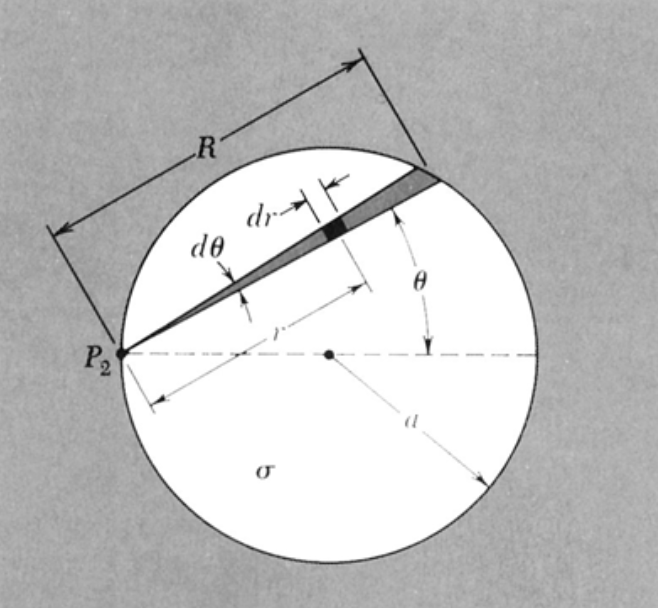
\includegraphics[width = 50mm]{ss11.png}
\end{center} 

An element of the wedge, the black patch at a distance $r$ from $P_2$ contains an an amount of charge $\sigma \, d\theta dr$. Its contribution to the Potential at $P_2$ is therefore just $\sigma d\theta dr$. The contribution of the entire wedge is then 

\[ \sigma d\theta \int_0^R dr = \sigma R d\theta \]\\

Now $R$ is $2a\cos\theta$ from the geometry of the right triangle, and the whole disk is swept out as $\theta$ ranges from $\frac{\pi}{2}$ to $\frac{\pi}{2}$. Thus the potential at $P_2$: 

\[ \phi = \int_{-\pi / 2}^{\pi / 2} 2\sigma a \cos \theta \, d\theta = 4\sigma a \] \\

Comparing this with $2\pi \sigma a$, the potential at the center of the disk, we see the potential falls from the center to the edge of the disk. The electric field therefore, must have an \textit{outward} component in the plane of the disk. That is why if a positive charge was free to move, it would redistribute itself to the rim. The uniformly charged disk is not a surface of constant potential. \\

The electric field on the symmetry axis can be computed directly from the potential function: 

\[ E_y = -\frac{d\varphi}{dy} = \frac{d}{dy} 2\pi \sigma (\sqrt{y^2 + a^2} - y) \] \\

giving 

\[ E_y = 2\pi \sigma \left[1 - \frac{y}{\sqrt{y^2+a^2}} \right] \hspace{20px} y > 0 \]\\

The energy associated with this electric field could be expressed as an integral over all space of $E^2 \, dv / 8\pi$. It is equal to the work done in assembling this distribution, starting with the infinitesimal charges far apart. \\ 

There is a general relatino between the work $U$ required to assemble a charge distribution $\rho (x, y, z)$ and the potential $\varphi(x, y, z)$ of that distribution: 

\[ U = \frac{1}{2} \int \rho \varphi \, dv \] \\ 

Therefore, the Potential Energy Equation from Chapter 1 could have been written this way instead, 

\[ \frac{1}{2} \sum_{j=1}^N q_j \sum_{k\neq j} \frac{q_k}{r_{jk}} \] \\

The second sum is the potential at the location of the $j$th charge, due to all the other charges. To adapt this to a continuous distribution of charge, we mereley replace $q_j$ with $\rho \, dv$ and the sum over $j$ by an integral, thus obtaining the previous integral. \\

\subsection{Divergence of a Vector Function} 

The electric field is a vector function of coordinates, $\vec{E}(x, y, z)$. \\ 

Consider a finite volume $V$ of some shape, the surface of which we shall denote by $S$. We already are familar with the notion of total flux $\Phi$ emerging from S. It is the value of 

\[ \int_S \vec{E} \cdot d\vec{a} \] \\

In the integrand, $d\vec{a}$ is the infinitesimal vector whos magnitude is the area of a small element of $S$ and whose direction is the outward-pointing normal to that little patch of the surface. \\

Now imagine dividing $V$ into two parts by a surface, $D$ that cuts throughg the ``ballon'' $S$. denote the two parts of $V$ by $V_1$ and $V_2$, treating them as distinct volumes, and compute the surface integral separately. 

\begin{center}
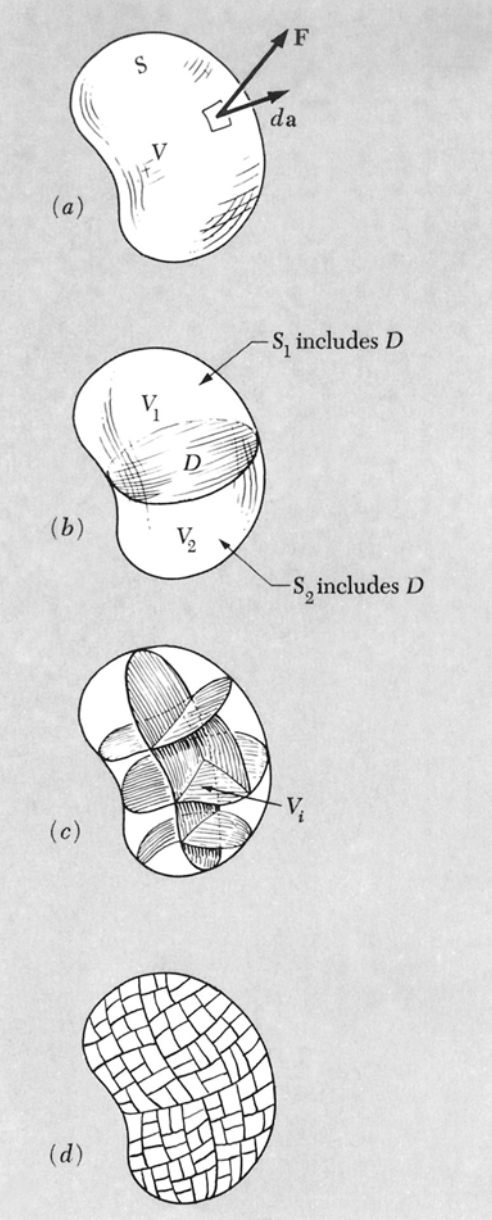
\includegraphics[width = 50mm]{ss12.png}
\end{center} 


Therefore, 

\[ \int_S \vec{E} \cdot d\vec{a} = \int_{S_1} \vec{E} \cdot d\vec{a_1} + \int_{S_2} \vec{E} \cdot d\vec{a_2} \] \\ 

Therefore, 

\[ \sum_{i=1}^N \int_{S_i} \vec{E} \cdot d\vec{a_i} = \int_S \vec{E} \cdot d\vec{a} = \Phi \] \\ 

Since you can just make an infinite number of separate volumes and surface integrals and add them to make the original surface integral. In the limit as $N$ becomes enormous, let us identify a characteristic of a particular small region, -- and ultimately, of the neighborhood of a point.  

If we keep halfing volumes creating smaller $V_i$s, we notice that summing all the volumes leads back to the original volume as well. This suggests us to look at the \textit{ratio} between the surface integral and a volume of an element in the subdivided space: 

\[ \frac{\int_{S_i} \vec{E} \cdot d\vec{a_i}}{V_i} \] \\

It seems plausible that for $N$ large enough, that is, for sufficiently fine-grained subdivision, we can halve the volume every time we halve the surface integral so that we shall find that with continuing subdivision of any particular region this ratio approaches a limit. If so, this limit is a property characteristic of any vector function \textbf{F} in that neighborhood. We call this limit, the \textit{the divergence} of \textbf{F}, written $\text{div} \vec{F}$. Therefore the value of div \textbf{E} at any point is defined as 

\[ \text{div} \vec{E} \equiv \lim_{V_i \to 0} \frac{1}{V_i} \int_{S_i} \vec{E} \cdot d\vec{a_i} \] \\

The meaning of div \textbf{E} can be expressed in this way: div \textbf{E} is the flux out of $V_i$ per unit of volume, in the limit of infinitesimal $V_i$. It is a scalar quantity. Another way to calculate div \textbf{E} is simply 

\[ \text{div} \textbf{E} = \frac{\partial E}{\partial x} + \frac{\partial E}{\partial y} + \frac{\partial E}{\partial z} \]\\

\textbf{or} 

\[ \text{div} \textbf{E} = \nabla \cdot \vec{E} \] \\

\subsection{Gauss's Theorem and the Differential Form of Guass's Law}

Using the \textit{divergence theorem} from multivariable calculus, \\

\[ \iint_S \vec{E} \cdot d\vec{a} = \iiint_V \text{div} \vec{F} \, dv \]\\ 

Therefore,  \\

\[ \text{div} \vec{E} = 4 \pi k \rho = \frac{Q}{\epsilon_0} \] \\

\textbf{Differential Form of Gauss' Theorem} 

\[ \nabla \cdot \vec{E} = \frac{Q}{\epsilon_0} \] \\ 

\subsection{The Laplacian} \mbox{} \\ 

We have now met two scalar functions related to the electric field, $\varphi$ and div \textbf{E}. \\

Since $\vec{E} = -\nabla \varphi$, 

\[ \text{div} \vec{E} = - \text{div} \nabla \varphi = -\left(\frac{\partial^2 \varphi}{\partial x^2} + \frac{\partial^2 \varphi}{\partial y^2} + \frac{\partial^2 \varphi}{\partial z^2}\right) \] \\

The operation on $\varphi$ except for the minus sign which is basically ``div grad'' is known as the \textit{Laplacian}, the expression 

\[ \frac{\partial^2}{\partial x^2} + \frac{\partial^2 }{\partial y^2} + \frac{\partial^2}{\partial z^2} \] \\ 

This expression is the same thing as $\nabla^2$, and is therefore known as the \textit{Laplacian}. \\

Therefore, from Gauss' Law in differential form, we have 

\[ \nabla^2 \varphi = -4\pi k \rho = -\frac{Q}{\epsilon_0} \] 


\subsection{Laplace's Equation}

Wherever $\rho = 0 $, that is, in all parts of space containing no electric
charge, the electric potential  $\varphi$ has to satisfy the equation \[
\nabla^2 \varphi = 0
.\] \\

This is called \textit{Laplace's Equation}. The class of functions that satisfy
Laplace's Equations are called \textit{harmonic functions}. They have
remarkable properties, one of which is this: 

\begin{theorem}
  If $\varphi(x,y,z)$ satisfies Laplace's Equation, then the average value of
  $\varphi$ over the surface of any sphere is equal to the value of $\varphi$
  at the center of the sphere.
\end{theorem}

This can easily be proved as true for electric potential $\phi$ in regions
containing no charge. Consider a point charge $q$ and a spherical surface $S$
over which a charge $q'$ is uniformly distributed. Let the charge $q$ be
brought in from an infinite distance to  $R$ from the center of the charged
sphere. 

\begin{center}
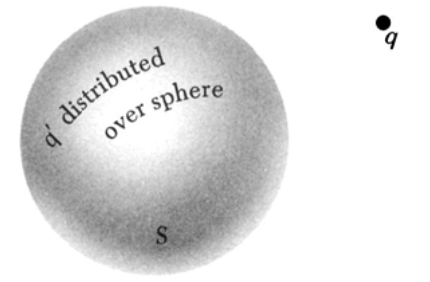
\includegraphics{screenshot 3.png}
\end{center}

The electric field of the sphere being the same as if its total charge $q'$
were concentrated in the center, the work required to bring $q$ from infinity
to $R$ is $\frac{qq'}{R}$. Now suppose instead, that the point charge $q$ was
there first and the charged sphere was later brought in from infinity. The work
required for that is the product of $q'$ and the average over the surface $S$
of the potential due to the point charge $q$. The work is surely the same --
$\frac{qq'}{R}$, so the average over the sphere of the potential due to $q$
must be $\frac{q}{R}$. This proves the assertion for any single point outside
the sphere. 

\subsection{Review so far} 
\vspace{20px}
\begin{center}
  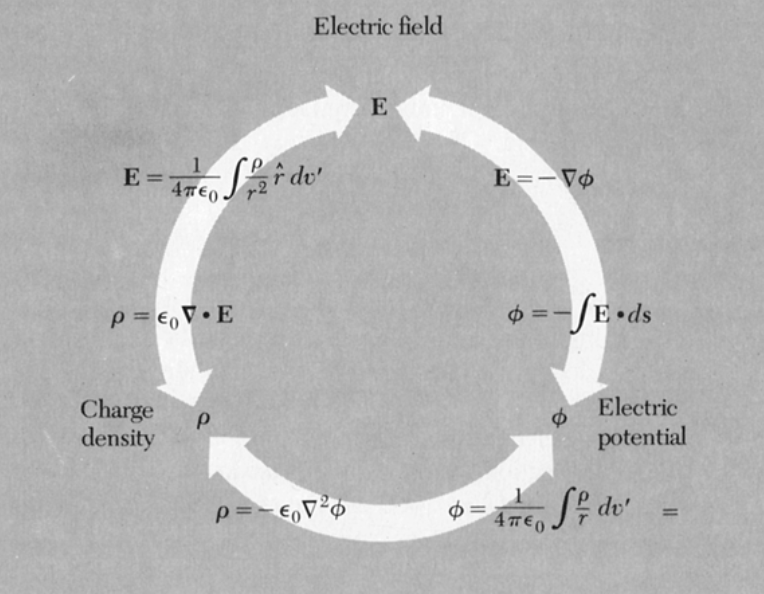
\includegraphics[width = 10cm]{screenshot 4.png}
\end{center}

\vspace{20px}

\subsection{Curl of a Vector Field}

The curl of a vector field is defined as \[
  \text{curl} \textbf{F} = \text{det} \begin{pmatrix}
    \hat{i} & \hat{j} & \hat{k} \\
    \frac{\partial}{\partial x} & \frac{\partial}{\partial y}
                                & \frac{\partial}{\partial z} \\
    P & Q & R 
  \end{pmatrix}
.\] \\
where $P, Q, R$ are the components of a vector field $F$ \\

This equation can be simplified as 

\[
  \text{curl } \textbf{F} = \nabla \cdot \textbf{F}   
.\] 


\subsection{Stokes' Theorem}

\[ \int_C \vec{F} \cdot d\vec{s} = \iint_S \text{curl} \vec{F} \cdot d\vec{a}
\] \\

This means you can convert a single line integral into a double integral if the
vector function is a 3 dimensional one. 

\subsection{The Physical Meaning of Curl}


The name \textit{curl} reminds us that the vector field with a nonezero curl
has a circulation, or vorticity. Maxwell used the name \textit{rotation}\\

\begin{figure}
  \centering
  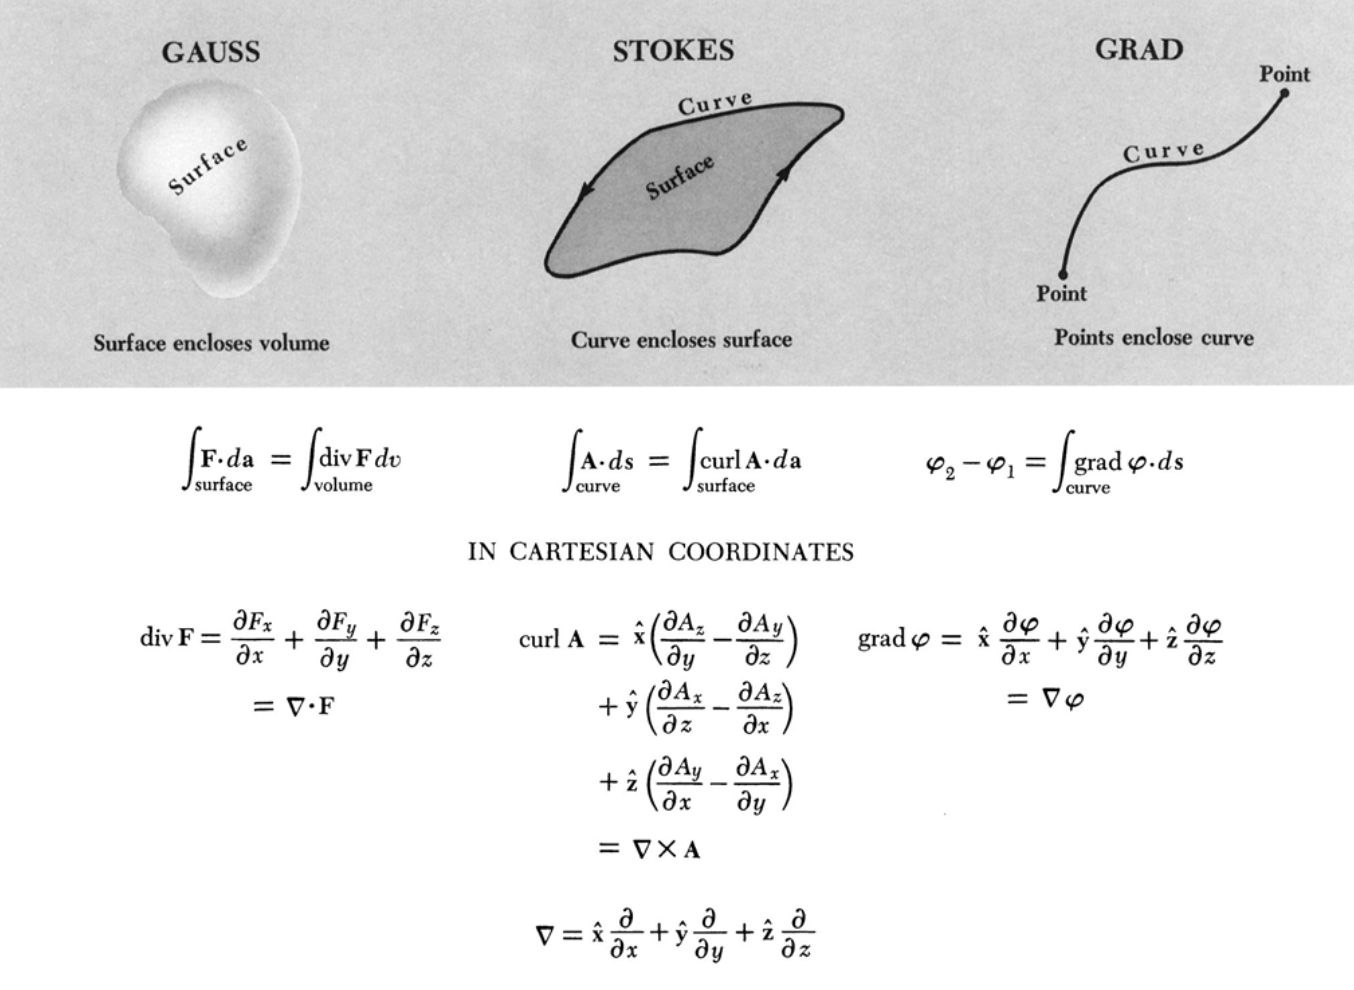
\includegraphics[width = 15cm]{screenshot 5.png}
  \caption{Some Vector Relations Summarized}
\end{figure}

\section{Electric Fields Around Conductors}

The electrical difference between a good conductor and a good insulator is as
vast as the mechanical difference between a solid and a liquid. That is not
entirely accidental. Both properties depend on the \textit{mobility} of atomic
particles: in the electrical case, the mobility of the carriers of charge,
electrons or ions; in the case of the mechanical properties, the mobility of
atoms or molecules make up the structure of the material. 

\subsection{Conductors in the Electrostatic Field}

\vspace{20px}
We shall be interested in the \textit{stationary} state of charge and electric
field that prevails after all redistributions of charge have taken place in the
conductors. \\

For example, bring in two charged metal spheres, insulated from one another,
and from everything else. Fix them in positions relatively near one another.
What is the resulting electric field in the whole space surrounding and between
the spheres, and how is the charge that was on each sphere distributed? We
begin with a more general question: After the charges have become stationary,
what can we say about the electric field inside conducting matter? \\

Positive ions are drawn in one direction by the field, and negative ions in the
opposite direction. They can go no farther than the surface of the conductor.
Piling up there, they begin to themselves create an electric field inside the
body which tends to \textit{cancel} the original field. And in fact, the
movement goes until that original field is \textit{precisely} canceled. The
final distribution of charge at the surface, is therefore such that its field
and the field of the external sources combine to give \textit{zero} electric
field in the interior of the conductor. 

\begin{center}
  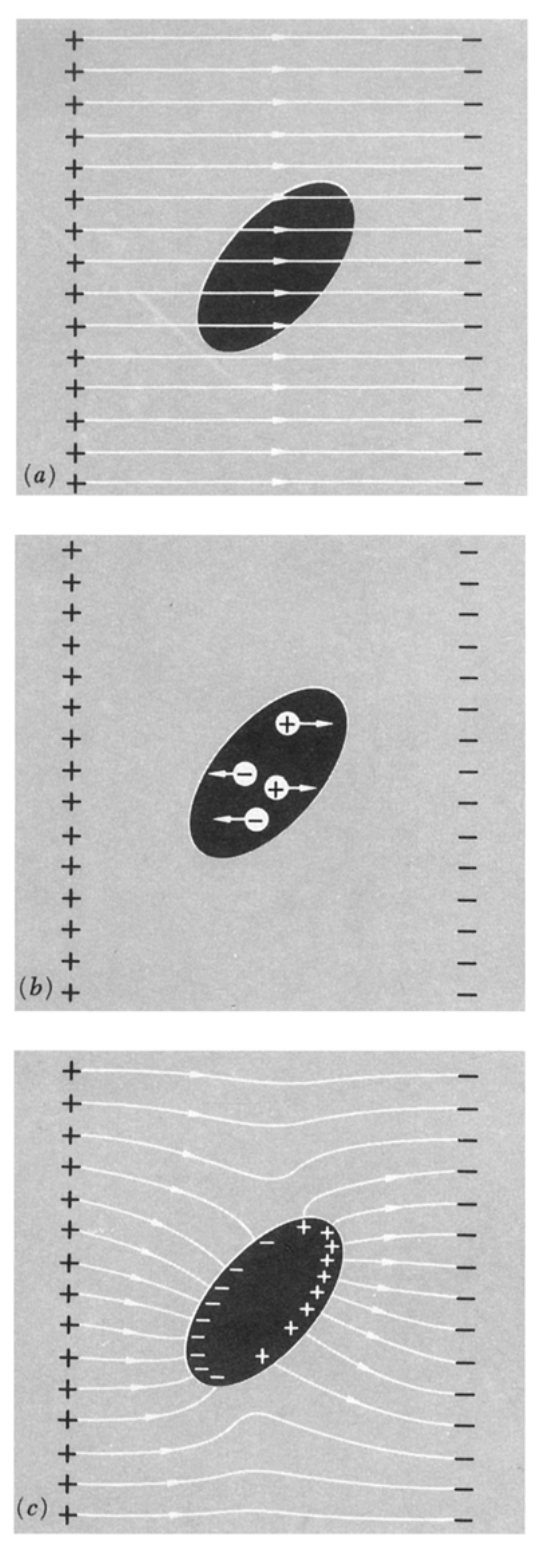
\includegraphics[width = 5cm]{screenshot 6.png}
\end{center}

Because the surface of a conductor is necessarily a surface of constant
potential, the electric field, which is $-\nabla \varphi$ must be
\textit{perpendicular} to the surface at every point on the surface. Proceeding
from the interior of the conductor outward, we find at the surface an abrupt
change in the electric field;  \textbf{E} is not zero outside the surface, and
is zero inside. The discontinuity in \textbf{E} is accounted for by the
presence of surface charge, of density $\sigma$, which we can relate directly
to  \textbf{E} by Gauss' Law. (shown in the textbook). However, it is obvious
that the surface charge must account for the whole charge $Q_k$. That is, the
surface integral of $\sigma$ over the whole conductor must equal $Q_k$. In
summary, we can make the following statements about \textit{any} such system of
conductors. \\\[
\varphi = \varphi_k \text{ at all points on the surface of the $k$th conductor}
.\]\\ 

At any point just outside the conductor, \textbf{E} is perpendicular to the
surface, and $E = 4\pi k \sigma$. Therefore, 

\[
  Q_k = \int_{S_k} \sigma \, da = \frac{1}{4\pi} \int_{S_k} \vec{E} \cdot
  d\vec{a} 
\]\\
\begin{center}
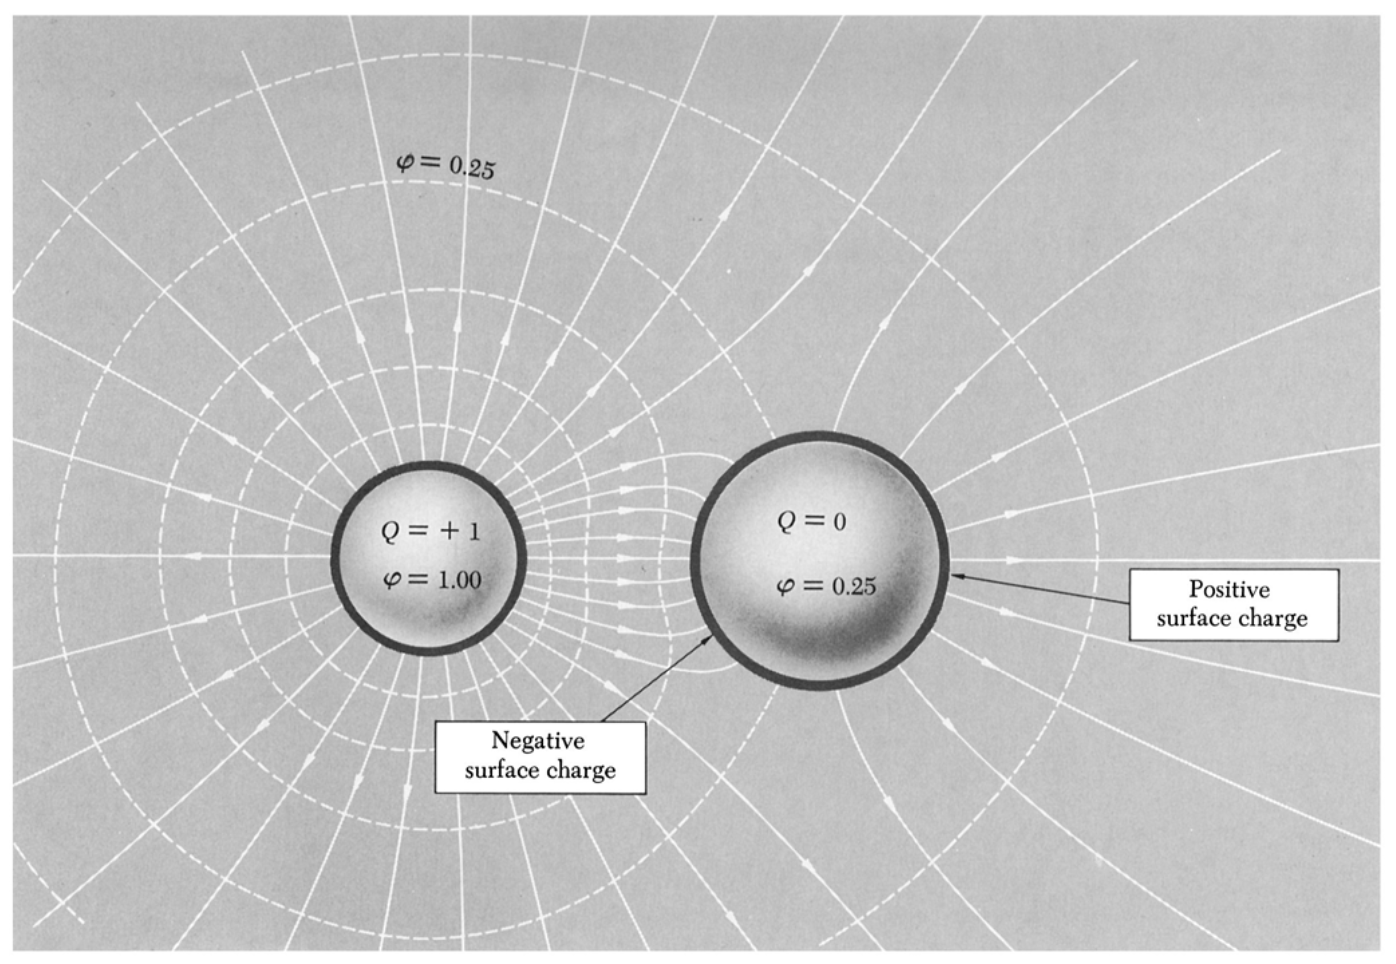
\includegraphics[width = 15cm]{screenshot 7.png}
\end{center}

The electric field around two spherical conductors, one with total charge 1,
and one with total charge 0. Dashed curves are intersections of equipotential
surfaces with the plane of the figure. 

\subsection{The General Electrostatic Problem; Uniqueness Theorem}

Everywhere outside the conductors, $\nabla^2 \varphi = 0$. Written out in
cartesian coordinates, 

\[
\frac{\partial^2\varphi}{\partial x^2} + \frac{\partial^2\varphi}{\partial y^2}
+ \frac{\partial^2\varphi}{\partial z^2} = 0
.\] \\

The problem is to find a function that satisfies the equation and also
satisfies the specified conditions on the conducting surfaces. Our solution
$\varphi (x,y,z)$ has to assume the correct value at all the points on each of
the surfaces. These surfaces in their totality \textit{bound} the region in
which $\varphi$ is defined, if we include a large surfaces "at infinity," where
we require $\varphi$ to approach zero. Sometimes the region of interest is
totally enclosed by a conducting surface; then, we can assign the conductor
a potential and ignore anything outside it. In either case, we have a typical
\textit{boundary-value problem}, in which the value the function has to assume
on the boundary is specified for the entire boundary.\\

Assume there is another function $\psi(x,y,z)$ which is also a solution
meeting the same boundary conditions. Now, Laplace's Equation is
\textit{linear}. That is, if $\varphi$ and $\psi$ satisfy Laplace's
Equation, then so does $c_1\varphi + c_2\psi$, where $c_1$ and $c_2$ are
constants. In particular, the difference between our two solutions, $\varphi
- \psi$, must satisfy Laplace's Equation. Call this function $W$. 

\[
W(x,y,z) = \varphi(x,y,z) - \psi(x,y,z)
.\] 

Of course, $W$ does not satisfy the boundary conditions. In fact, the surface
of every conductor $W$ is zero, because $\psi$ and $\varphi$ take on the same
value, $\varphi_k$ at the surface of a conductor $k$. Thus, $W$ is a solution
of \textit{another} electrostatic problem, one with the same conductors but
with all conductors held at zero potential. \\

We can now demonstrate easily that 

\begin{theorem}
  In the space inside a hollow conductor of any shape whatever, if that space
  itself is empty of charge, the electric field is zero.
\end{theorem} 

This is true whatever the field may be outside the conductor. This is because
the potential function inside the box, $\varphi(x,y,z)$, must satisfy Laplace's
Equation. The entire boundary of a conductor, is an equipotential, so we have
$\varphi = \varphi_0$, a constant everywhere on the boundary. Since $\varphi$
is a constant, \textbf{E} $= 0$, since $\vec{E} = -\nabla \varphi$. 





\end{document}
